\documentclass[12pt]{article}
\usepackage{amsmath, graphicx}
\usepackage[french]{babel}
\usepackage[top=2.3cm, bottom=2.3cm, left=2.5cm, right=2.5cm]{geometry}

\begin{document}

\begin{titlepage}
    \begin{center}
        \vspace*{1cm}
            
        \Huge
        \textbf{Rapport de projet}
            
        \vspace{0.5cm}
        \LARGE
        Traitement de l'information
            
        \vspace{1.5cm}
        
        \hrule
        \vspace{0.5cm}
        \textbf{Léo Paillé - Gatien Menaud - Alix Renoncourt}
        \vspace{0.5cm}
        \hrule
            
        \vspace{2cm}
            
        \Large
        EI5IS102 - Traitement de l’Information\\
        Département informatique\\
        S5 - 2023/2024
        
        \vfill
            
        
\includegraphics[width=0.4\textwidth]{./utils/Logo_enseirb.png}
        
    \end{center}
    
        \small
        ENSEIRB-MATMECA, Bordeaux, 10 Janvier 2024
        \normalsize
            
\end{titlepage}

\tableofcontents

\newpage

\section{Introduction}

Dans ce rapport, nous allons présenter les données que nous avons décidé de traiter, la méthode de traitement utilisée, puis l'analyse des résultats obtenus.\\
Notre objectif est de créer un modèle de génération de texte, entraîné auparavant depuis une base de données textuelles. Pour cela, nous nous appuyons en partie sur le modèle de langage GPT (transformateur génératif pré-entraîné), développé par OpenAI, ainsi que d'autres projets collaboratifs communautaires, tel que Llama2(?) %+Lien?.

\section{Présentation des données}

Pour créer un modèle capable de générer du texte à partir d'un mot ou d'une phrase (appelé \textit{prompt}), il est tout d'abord nécessaire d'entraîner ce modèle à partir de texte préexistant. Plus l'échantillon de texte est grand, plus la réponse générée pourra être complète, diversifiée et cohérente. Nous décidons pour cela de récupérer un jeu de données \textit{TinyStories.txt\footnotemark[1]} (une fois décompressé), contenant plusieurs histoires de quelques lignes, en anglais, totalisant plus de 1.6G de caractères. Notez qu'une partie non négligeable de ces textes a été elle-même générée par les modèles GPT-3.5 et GPT-4. Voici un échantillon du jeu de données en figure \ref{fig:echantTS} : 

\begin{figure}[h]
	\centering
    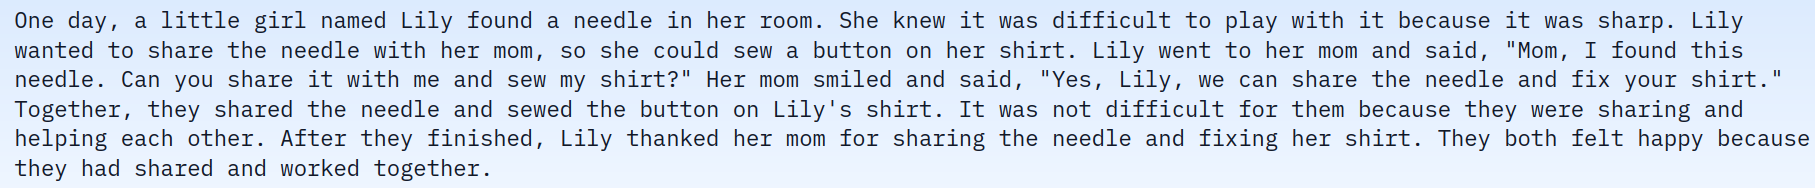
\includegraphics[scale=0.26]{./utils/EchantillonTinyStories.png}
    \caption{\textit{Échantillon de TinyStories.txt}}
    \label{fig:echantTS}
\end{figure}

\section{Présentation de la méthode}

\subsection{Entraînement du modèle}

À présent que nous avons un ensemble de données sur lesquelles travailler, il faut entraîner notre modèle. L'objectif étant de générer du texte lisible et cohérent, notre programme doit être capable de déterminer, à partir d'une phrase ou un mot, une suite à celui-ci. Nous devons donc lui apprendre les liens qui peuvent exister entre plusieurs groupes de mots ou de lettres, provenant d'une phrase courante depuis notre base de donnée. Dans son état final, notre modèle sera une matrice de flottants, chacun correspondant à la cohérence entre un groupe de caractères et un caractère particulier, soit la probabilité qu'un certain caractère se trouve après une suite de plusieurs autres.\\

Pour cela, nous allons en premier découper notre base de donnée en petites portions de texte pour ne pas surcharger l'espace de mémoire lors de l'entraînement. Ensuite, pour chacun de ces bouts de texte, nous répétons un nombre défini de fois (\textit{n\_vocab}) l'opération suivante :\\
- Récupérer une chaîne de caractères \textit{s} à un emplacement aléatoire du texte, de longueur \textit{context\_size}\\
- Comparer la chaîne $s[1:context\_ size-1]$ avec le caractère $s[context\_ size]$ avec \textit{gzip}\\
- Répéter l'opération en tronquant s par la droite jusqu'à ce que $len(s) = 2$, de manière à avoir des données pour des échantillons de taille 1 à $context\_ size-1$\\

Les données de comparaison obtenues sont ensuite stockées dans la matrice. Par ailleurs, on conserve également toutes les chaînes \textit{s} dans une liste, pour pouvoir les réutiliser lors de l'exécution du programme, et savoir à quelle chaîne de caractères correspond chaque ligne de la matrice.\\

Ces opérations peuvent ensuite être répétées pour chaque portion de texte, mais cela requiert beaucoup de ressources, notamment liées au matériel utilisé (CPU), et donc de beaucoup de temps. Plus le modèle est entraîné, plus il sera capable de générer du texte cohérent et diversifié.\\

\subsection{Utilisation du modèle}

Une fois que l'on a obtenu notre matrice correspondant à notre modèle, il est simple et rapide de faire générer du texte par un programme prenant en entrée un prompt écrit par l'utilisateur, ainsi que notre modèle, et générant en sortie du texte. Ce texte se développe alors caractère par caractère de la manière suivante :\\
- Le programme récupère les $max(taille\_prompt$, $context\_size)$ derniers caractères du prompt\\
- Il regarde dans le modèle à quelle ligne correspond la chaîne de caractère ainsi étudiée\\
- Il choisit le caractère pour lequel la valeur dans la matrice est la plus grande (ou bien un caractère aléatoirement parmi tous ceux pour lesquels la valeur est supérieure à un nombre prédéfini)\\
- Il affiche ce caractère, puis réitère l'opération jusqu'à une condition d'arrêt (fin de phrase, nombre de caractères requis par l'utilisateur atteint, arrêt forcé...)\\

\section{Analyse du modèle et des résultats}

Le modèle que nous obtenons est satisfaisant, à partir d'un certain nombre d’entraînements. En effet, si le modèle n'est entraîné que sur une partie restreinte de texte, le programme risque de de ne pas avoir assez de données pour générer du texte, et donc de se répéter, voire de générer du texte illisible.\\



\section{Conclusion}

\section{Références}

\footnote[1]{huggingface.co/datasets/roneneldan/TinyStories}

\end{document}